\section{Results}
\label{sec:results}

\begin{table*}[t]
\centering\small
\setlength{\tabcolsep}{6pt}
\begin{tabular}{lcccc}
\toprule
 & \multicolumn{3}{c}{Llama-3.2-1B} & Qwen3-0.6B \\
\cmidrule(lr){2-4}\cmidrule(lr){5-5}
 & \multicolumn{2}{c}{main runs} & warm-up runs & main runs \\
\cmidrule(lr){2-3}\cmidrule(lr){4-4}\cmidrule(lr){5-5}
 & registered prefix & training separator & training separator & (both identical) \\
\midrule
\multicolumn{5}{l}{\emph{Held-out Nepali BPB} (lower is better)} \\
Base model, no training & 0.766 & n/a & n/a & 0.852 \\
\RO{} & 0.474 & 0.471 & 0.471 & 0.501 \\
\RI{} & 0.534 & 0.483 & 0.480 & 0.561 \\
\RII{} & 0.539 & 0.510 & 0.501 & 0.570 \\
\midrule
\multicolumn{5}{l}{\emph{Paired difference in held-out Nepali BPB} (positive: first arm worse), document-clustered 95\% interval} \\
\RI{} $-$ \RO{} & +0.060 & +0.012 & +0.010 & +0.060 \\
 & [+0.058, +0.061] & [+0.011, +0.013] & [+0.009, +0.011] & [+0.058, +0.062] \\[2pt]
\RII{} $-$ \RO{} & +0.066 & +0.039 & +0.031 & +0.070 \\
 & [+0.064, +0.068] & [+0.038, +0.041] & [+0.029, +0.032] & [+0.067, +0.072] \\[2pt]
\RII{} $-$ \RI{} & +0.006 & +0.027 & +0.021 & +0.009 \\
 & [+0.004, +0.007] & [+0.026, +0.028] & [+0.020, +0.022] & [+0.008, +0.010] \\
\midrule
Training tokens (M), \RO{}/\RI{}/\RII{} & \multicolumn{3}{c}{417 / 386 / 286} & 574 / 392 / 292 \\
Decoding steps, relative to \RII{} & \multicolumn{3}{c}{2.55 / 2.17 / 1} & 4.35 / 2.16 / 1 \\
\bottomrule
\end{tabular}
\caption{Continued pretraining on the same 1\,GB of Nepali and 1\,GB of English in every arm (one run per arm). BPB: bits per byte on held-out native Nepali, scored in pieces of about 2{,}000 bytes. Registered prefix: the beginning-of-sequence token, as pre-registered. Training separator: the end-of-text token that preceded every document during training (a post hoc diagnostic). Qwen has no beginning-of-sequence token, so both prefixes are the end-of-text token. Intervals resample 484 documents (2{,}259 pieces; a piece shorter than 1{,}900 bytes is taken to end a document) and reflect only the sampling of evaluation text. Warm-up runs under the registered prefix and all secondary metrics are in Table~\ref{tab:cpt}. Decoding steps: tokens needed for FLORES-200 Nepali devtest, relative to \RII{}.}
\label{tab:prefix}
\end{table*}


\subsection{Compression}
\label{sec:compression}

Figure~\ref{fig:ksweep} sweeps the number of new merges $K$. Under the letters-only regex (\RI{}), extension saturates almost at once. For Llama-3 the first 1{,}000 merges take the premium from $2.58$ to $2.32$, and the next 63{,}000 only to $2.20$, within $0.01$ of the floor. For Qwen3, \RI{} reaches $2.19$ by $K{=}16$k and stops at $2.18$, against a floor of $2.17$. It stops early because the letters-only regex leaves few distinct Nepali pre-tokens to merge (Appendix~\ref{app:extras}). Under the repaired regex (\RII{}), additional merges keep helping. At $K{=}32$k Nepali reaches parity with English ($1.01$) on both models, and at $64$k it is cheaper than English ($0.95$), below \texttt{o200k}. At $K{=}32$k, \RII{} needs 46\% of \RI{}'s tokens for FLORES Nepali. All 28 extended tokenizers decode losslessly and reproduce the original token ids on all 1{,}012 English devtest sentences, as \S\ref{sec:floor} and Proposition~\ref{prop:lossless} predict.

\begin{figure}[t]
\centering
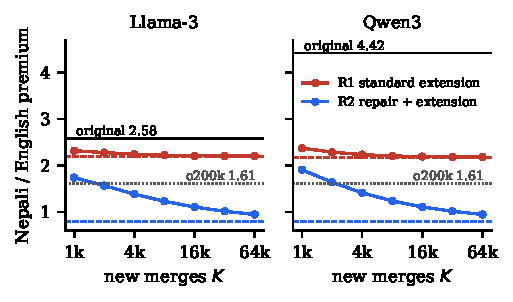
\includegraphics[width=\columnwidth]{fig_ksweep.pdf}
\caption{Nepali/English premium on FLORES-200 devtest after adding $K$ merges by continued BPE, under the letters-only regex (\RI{}) and the repaired regex (\RII{}). Dashed lines: pre-token floors under each model's own pattern ($2.19$ and $2.17$ letters-only; $0.79$ and $0.80$ repaired, for Llama-3 and Qwen3). 95\% paired-bootstrap intervals (half-width at most 0.03) are narrower than the markers.}
\label{fig:ksweep}
\end{figure}

Both parts of the repair are needed. Repairing the regex without new merges changes almost nothing ($2.61$ for Llama-3, $4.42$ for Qwen3), because the old merges still cut Nepali words into the old pieces. The repair also mends syllables. The share of Nepali tokens that start with a combining mark rises from 55\% (Llama-3) and 32\% (Qwen3) to 65\% and 64\% under \RI{}, since new merges can only build on mark-initial fragments, and falls to 13\% and 11\% under \RII{}.

We repeated the sweep for seven other languages written with combining marks and two controls (Table~\ref{tab:xling}, Appendix~\ref{app:xling}), learning merges on 25 to 361\,MB of FineWeb-2 text per language. At $K{=}32$k, \RII{} brings all seven to between $0.88$ and $1.24$ times English. \RI{} ends within 5\% of its floor in six of them. Thai is the exception: it is written without spaces, so its letters-only pre-tokens are long and leave \RI{} room. For Amharic and Korean, whose scripts have no combining marks, \RI{} and \RII{} are identical at every $K$, as the mechanism predicts.

\subsection{Continued pretraining}
\label{sec:cpt}

\paragraph{The registered outcome.} Table~\ref{tab:prefix} gives the results. The main hypothesis fails against \RO{}. Continued pretraining without new tokens gave the lowest held-out Nepali BPB on both models, and \RII{} was worse than \RO{} by $0.066$ on Llama and $0.070$ on Qwen, far beyond the 0.01 margin. Under this prefix standard extension also lost to \RO{}, by $0.060$ on both models. The new embeddings start as averages of existing ones, and 1\,GB of Nepali is not enough for them to catch up with tokens the base model already knows. Against standard extension, the registered comparison gives \RII{} $-$ \RI{} $= +0.0058$ $[+0.0044, +0.0073]$ for Llama, which is non-inferior, and $+0.0094$ $[+0.0084, +0.0104]$ for Qwen. The Qwen interval excludes zero and its upper end crosses the margin, so non-inferiority is not shown and \RII{} is worse. That verdict turns on 0.0004 BPB, a difference a second training run could plausibly move; we did not measure run-to-run variance.

\paragraph{The training separator.} For Llama, scoring after the training separator instead of BOS lowers BPB by $0.003$ for \RO{}, $0.051$ for \RI{} and $0.029$ for \RII{}, so the choice of first token changes the comparison. After the separator, \RII{} is worse than \RI{} by $+0.027$ $[+0.026, +0.028]$. We consider the separator scores closer to how the models were trained, but we chose them after seeing results, and BOS-prefixed inference is the default in Hugging Face and in chat templates, so the registered numbers are what a deployment would see. We have not established why the shift depends on the arm. With tied embeddings, the BOS row is updated as an output class even though it never appears as input, and in the warm-up runs its norm grows from $0.863$ to $0.896$ (Appendix~\ref{app:cptfull}); this may contribute. Training with BOS at every document start would remove the problem.

\paragraph{What the repair buys.} \RII{} trains on 26\% fewer tokens than \RI{} for the same bytes, but this does not make it cheaper to reach a given quality. At \RII{}'s final step count, the \RO{} checkpoint, whose learning rate had not yet decayed, is already better than the final \RII{} model by $0.060$ $[0.056, 0.063]$ on Llama and $0.053$ $[0.049, 0.057]$ on Qwen. The \RI{} checkpoint at that step is better by $0.006$ $[0.003, 0.008]$ on Llama and level on Qwen (scored on the first 1\,MB of held-out text, registered prefix). Measured training time fell by only 3\% (Llama) and 11\% (Qwen) relative to \RI{}, in runs that shared GPUs with evaluation jobs. The clear gain is at inference: for the same FLORES Nepali text, \RII{} needs $2.17$ (Llama) and $2.16$ (Qwen) times fewer decoding steps than \RI{}, which has the same vocabulary size, and $2.55$ and $4.35$ times fewer than \RO{}.

\paragraph{Warm-up runs.} Training only the embedding matrix first leaves \RO{} where it was ($0.471$ after the separator) and improves \RII{} from $0.510$ to $0.501$. \RII{}'s deficit relative to \RO{} shrinks from $0.039$ to $0.031$, as the second amendment predicted, and its gap to \RI{} from $0.027$ to $0.021$ $[0.020, 0.022]$. These are differences between single runs, so we treat them as suggestive. The amendment stated its prediction for the registered prefix, where the warm-up makes Llama scores unusable: \RO{} moves from $0.474$ to $0.779$.

\paragraph{English.} The registered English control holds. \RII{} $-$ \RO{} on held-out English is $+0.0003$ $[-0.0002, +0.0008]$ for Llama (non-inferior) and $-0.0028$ $[-0.0032, -0.0024]$ for Qwen (better), and no two main-run arms of a model differ by more than $0.004$. This is expected, since the tokenizer change does not touch English and every arm sees the same English data. Under the registered prefix all three Llama arms are slightly worse on English than the base model ($0.799$ to $0.803$ against $0.788$).
